
\section{Datasets}

In our approach we propose a supervised machine learning algorithm to estimate the page rank using deep graph networks. For this purpose we require labeled data to develop, train, and validate our model.

In general the process of gathering, augmenting, and labeling data can take an immense amount of time and can slow down the development of machine learning models. Therefore, we decided to iteratively develop and align our dataset to the current need of research and progress of development. For each upcoming iteration we specified the requirements for the dataset. Following from this, each iteration resulted in a corresponding dataset version.

The following sections will profoundly specify each dataset version as required during the development phase.

\subsection{Dataset Version 1}
\label{DatasetVersion1}
The dataset version 1 consists of 100,000 samples in total. The ground truth for this dataset version is OpenPage Rank, which is described in section \ref{OpenPageRank}.

Every sample $X$ is corresponds to a domain $D$ contained in the ground truth. We denote the $r$th sample as $X^{(r)}$. It can be expressed as a tuple consisting of four values:

\begin{center}
 $X^{(r)} = (\tensorsym{I}, r, u)$
\begin{itemize}
	\item[$\tensorsym{I}$] The screenshot of the domain $D$ in image format PNG and in the resolution $1920\times1080$. The image tensor has four channels, $\tensorsym{I}$ is therefore $\in\mathbb{R}^{1920\times1080\times4}$.
	\item[$r$] The global rank of the domain $D$, according to Open PageRank, within $[1, 100000]$. 
	\item[$u$] The URL of the domain $D$ mapped by the Open PageRank list. For example a string like \texttt{github.com}.
\end{itemize}
\end{center}

\subsection{Dataset Version 2}
\label{DatasetVersion2}
The dataset version 2 consists of 100,000 samples in total and the ground truth is \textit{Open PageRank} as described in dataset version 1.

Every sample $X$ is corresponds to a domain $D$ contained in the ground truth. We denote the $r$th sample as $X^{(r)}$. It can be expressed as a tuple consisting of four values:

\begin{center}
$X = (G,u,r,h)$
\begin{itemize}
    \item[$G$] The directed graph of the domain $D$ characterized by a set of nodes $\mathbb{V}$ and edges $\mathbb{E}$: $G= \left(\mathbb{V}, \mathbb{A}\right)$.
	\item[$u$] The URL of the domain $D$ mapped by the Open PageRank list.
	\item[$r$] The global rank of the domain $D$, according to Open PageRank, within $[1, 100000]$. 
    \item[$h$] Indicator for whether or not the website uses the protocol HTTPS, the value is $\in\left\{\text{true}, \text{false}\right\}$.
\end{itemize}
\end{center}

\subsubsection{The Directed Graph}
The directed graph provides a topological view on the given website by representing all associated web pages within the same domain as vertices and connections as arrows as in figure \ref{fig:PartialDirectedGraph_timodenk.com} exemplary illustrated. During the crawling process as described in \ref{Datacrawler} vertices and arrows of the graph are created and enriched with local information about the visited web pages.

The directed graph $G$ is characterized by a set of nodes $\mathbb{V}$ and edges $\mathbb{E}$. Each node $v \in \mathbb{V}$ represents a web page of the given domain associated with the graph. A node is characterized by the following tuple:

\begin{center}
$v = (u, \tensorsym{I}, \tensorsym{M},t, l, s)$
\begin{itemize}
	\item[$u$] The exact URL of the web page. Example: \textit{https://github.com/help}
	\item[$\tensorsym{I}$] The screenshot of web page in image format PNG and in the resolution 1920x1080.
	\item[$\tensorsym{M}$] The screenshot of web page in image format PNG and in mobile resolution TODO ZxY.
	\item[$t$] The title of web page as can be seen in the tabs bar of a common browser.
	\item[$l$] The time it takes to download all data of web page from the web server in milliseconds.
	\item[$s$] Number of kilobytes downloaded in total for web page (size).
\end{itemize}
\end{center}

Each edge represents a possible navigation from web page $v_1$ to $v_2$ in the graph $G$. It can be understood as a hyperlink or button found on web page $v_1$ (source), which points to $v_2$ (target) in the same domain. 

\begin{center}
	$v \in (v_1, v_2, t)$
	\begin{itemize}
		\item[$v_1$] The source node (web page).
		\item[$v_2$] The target node that $v_1$ points to.
		\item[$t$] If existent, the text that links from source to target web page.
	\end{itemize}
\end{center}

\begin{figure}
\centering
\usetikzlibrary{shapes.multipart}
  \tikzset{
	vertices/.style = {   
		text width=12.0em, align=center,                                           
		draw,
		rectangle split,
		rectangle split parts=6
	}
}
\scalebox{.85}{
\begin{tikzpicture}
\node[vertices]  (timodenk) at (5,4) {
	\nodepart{one} timodenk.com 
	\nodepart{two} 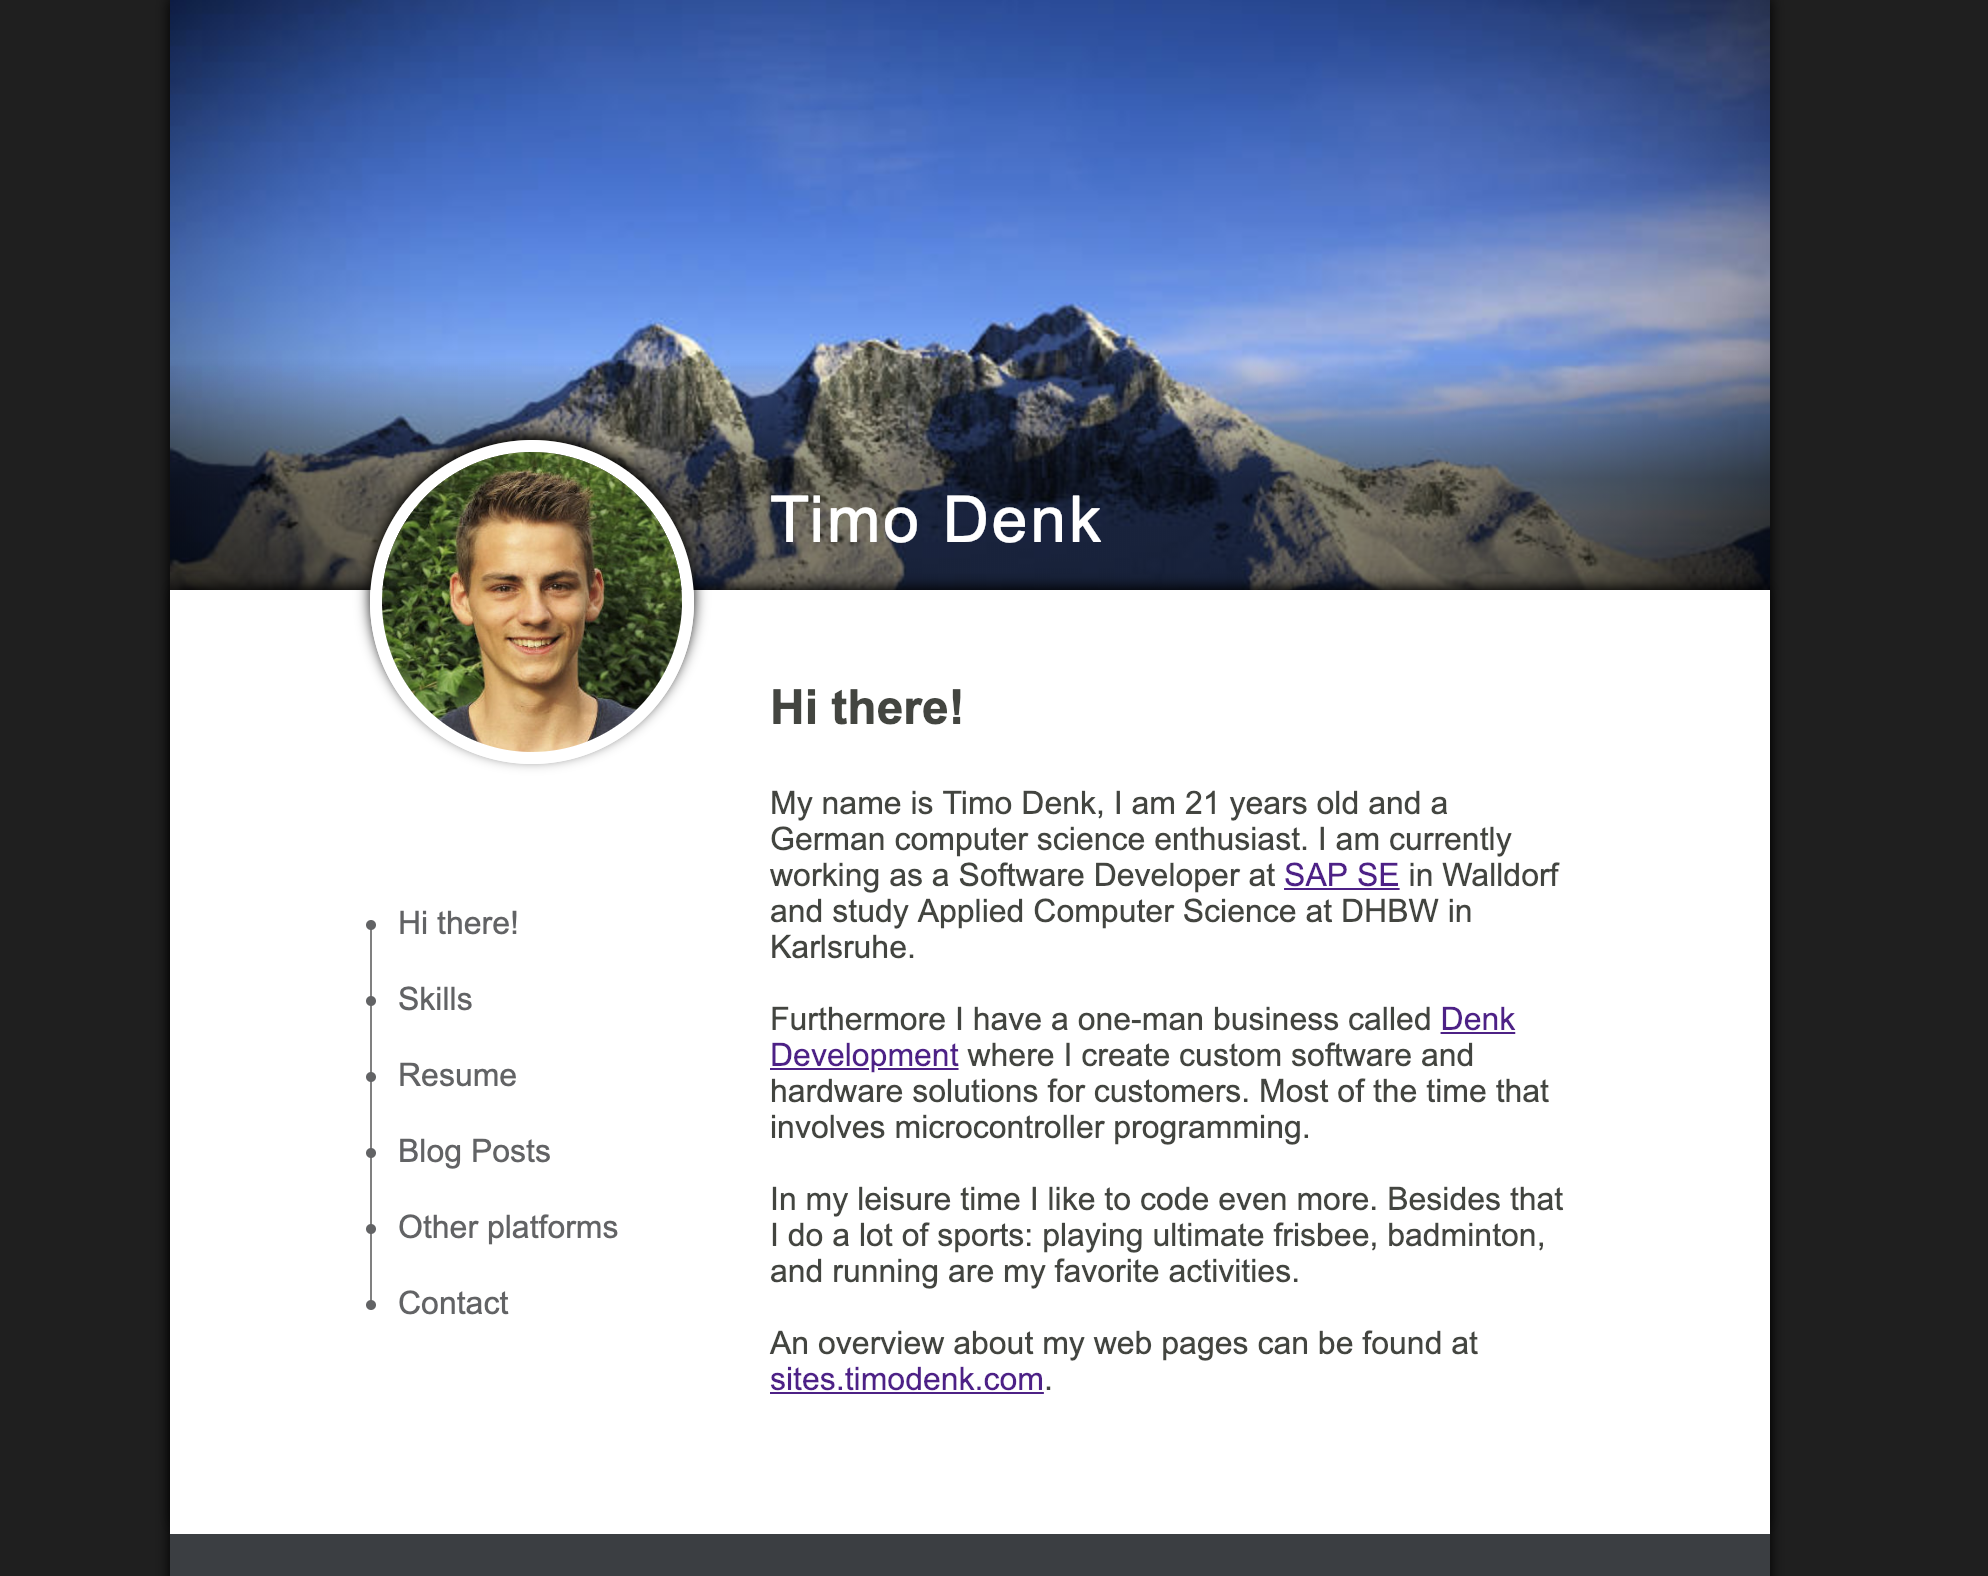
\includegraphics[width=.5\textwidth]{resources/timodenk}
	\nodepart{three} 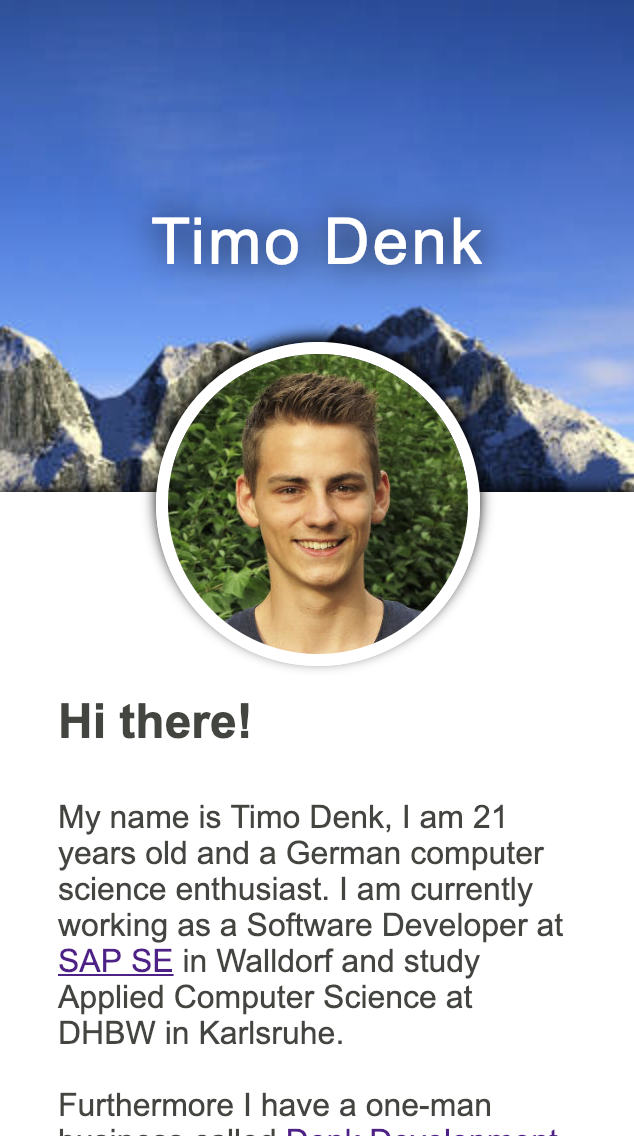
\includegraphics[width=.25\textwidth]{resources/timodenk_mobile}
	\nodepart{four} Timo Denk
	\nodepart{five} 636 ms
	\nodepart{six} 434 kb
};

\node[vertices]  (sites) at (10,2) {
\nodepart{one} sites.timodenk.com
\nodepart{two} 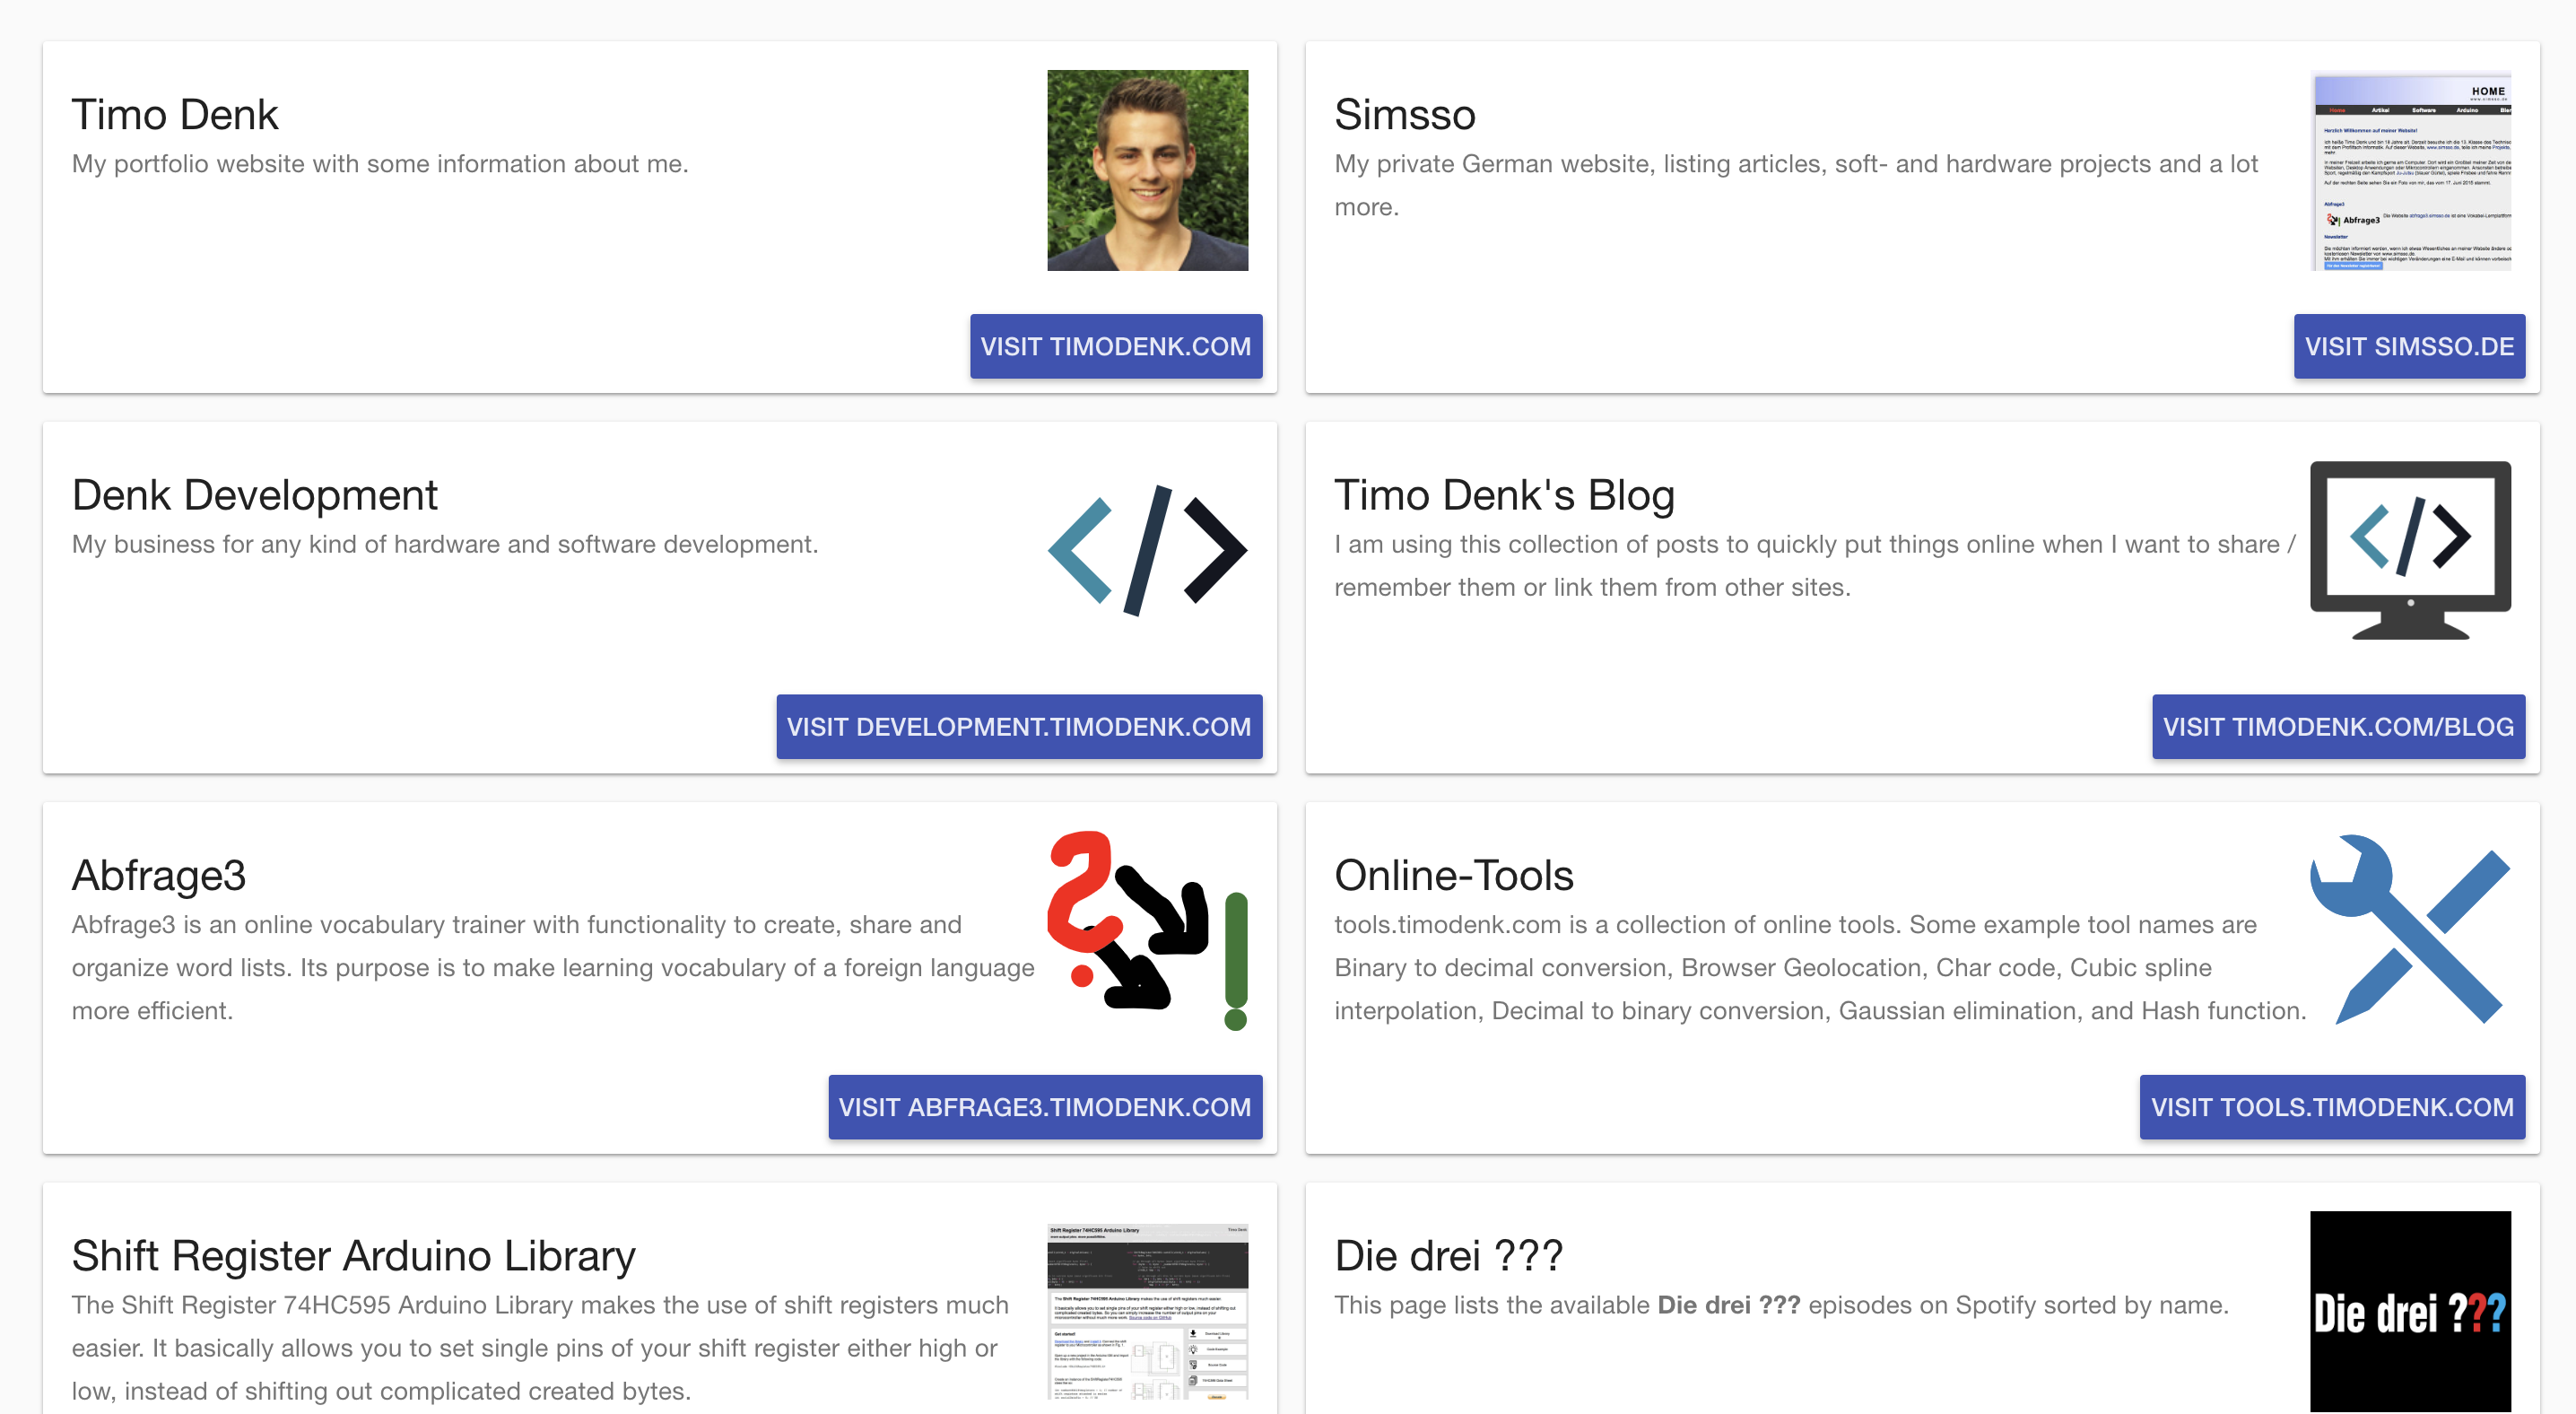
\includegraphics[width=.5\textwidth]{resources/sites_timodenk}
\nodepart{three} 
\includegraphics[width=.25\textwidth]{resources/sites_timodenk_mobile}	\nodepart{four} Timo Denk Sites Overview
\nodepart{five} 767 ms
\nodepart{six} 737 kb
};

\node[vertices]  (imprint) at (0,2) {
\nodepart{one} timodenk.com/imprint
\nodepart{two} 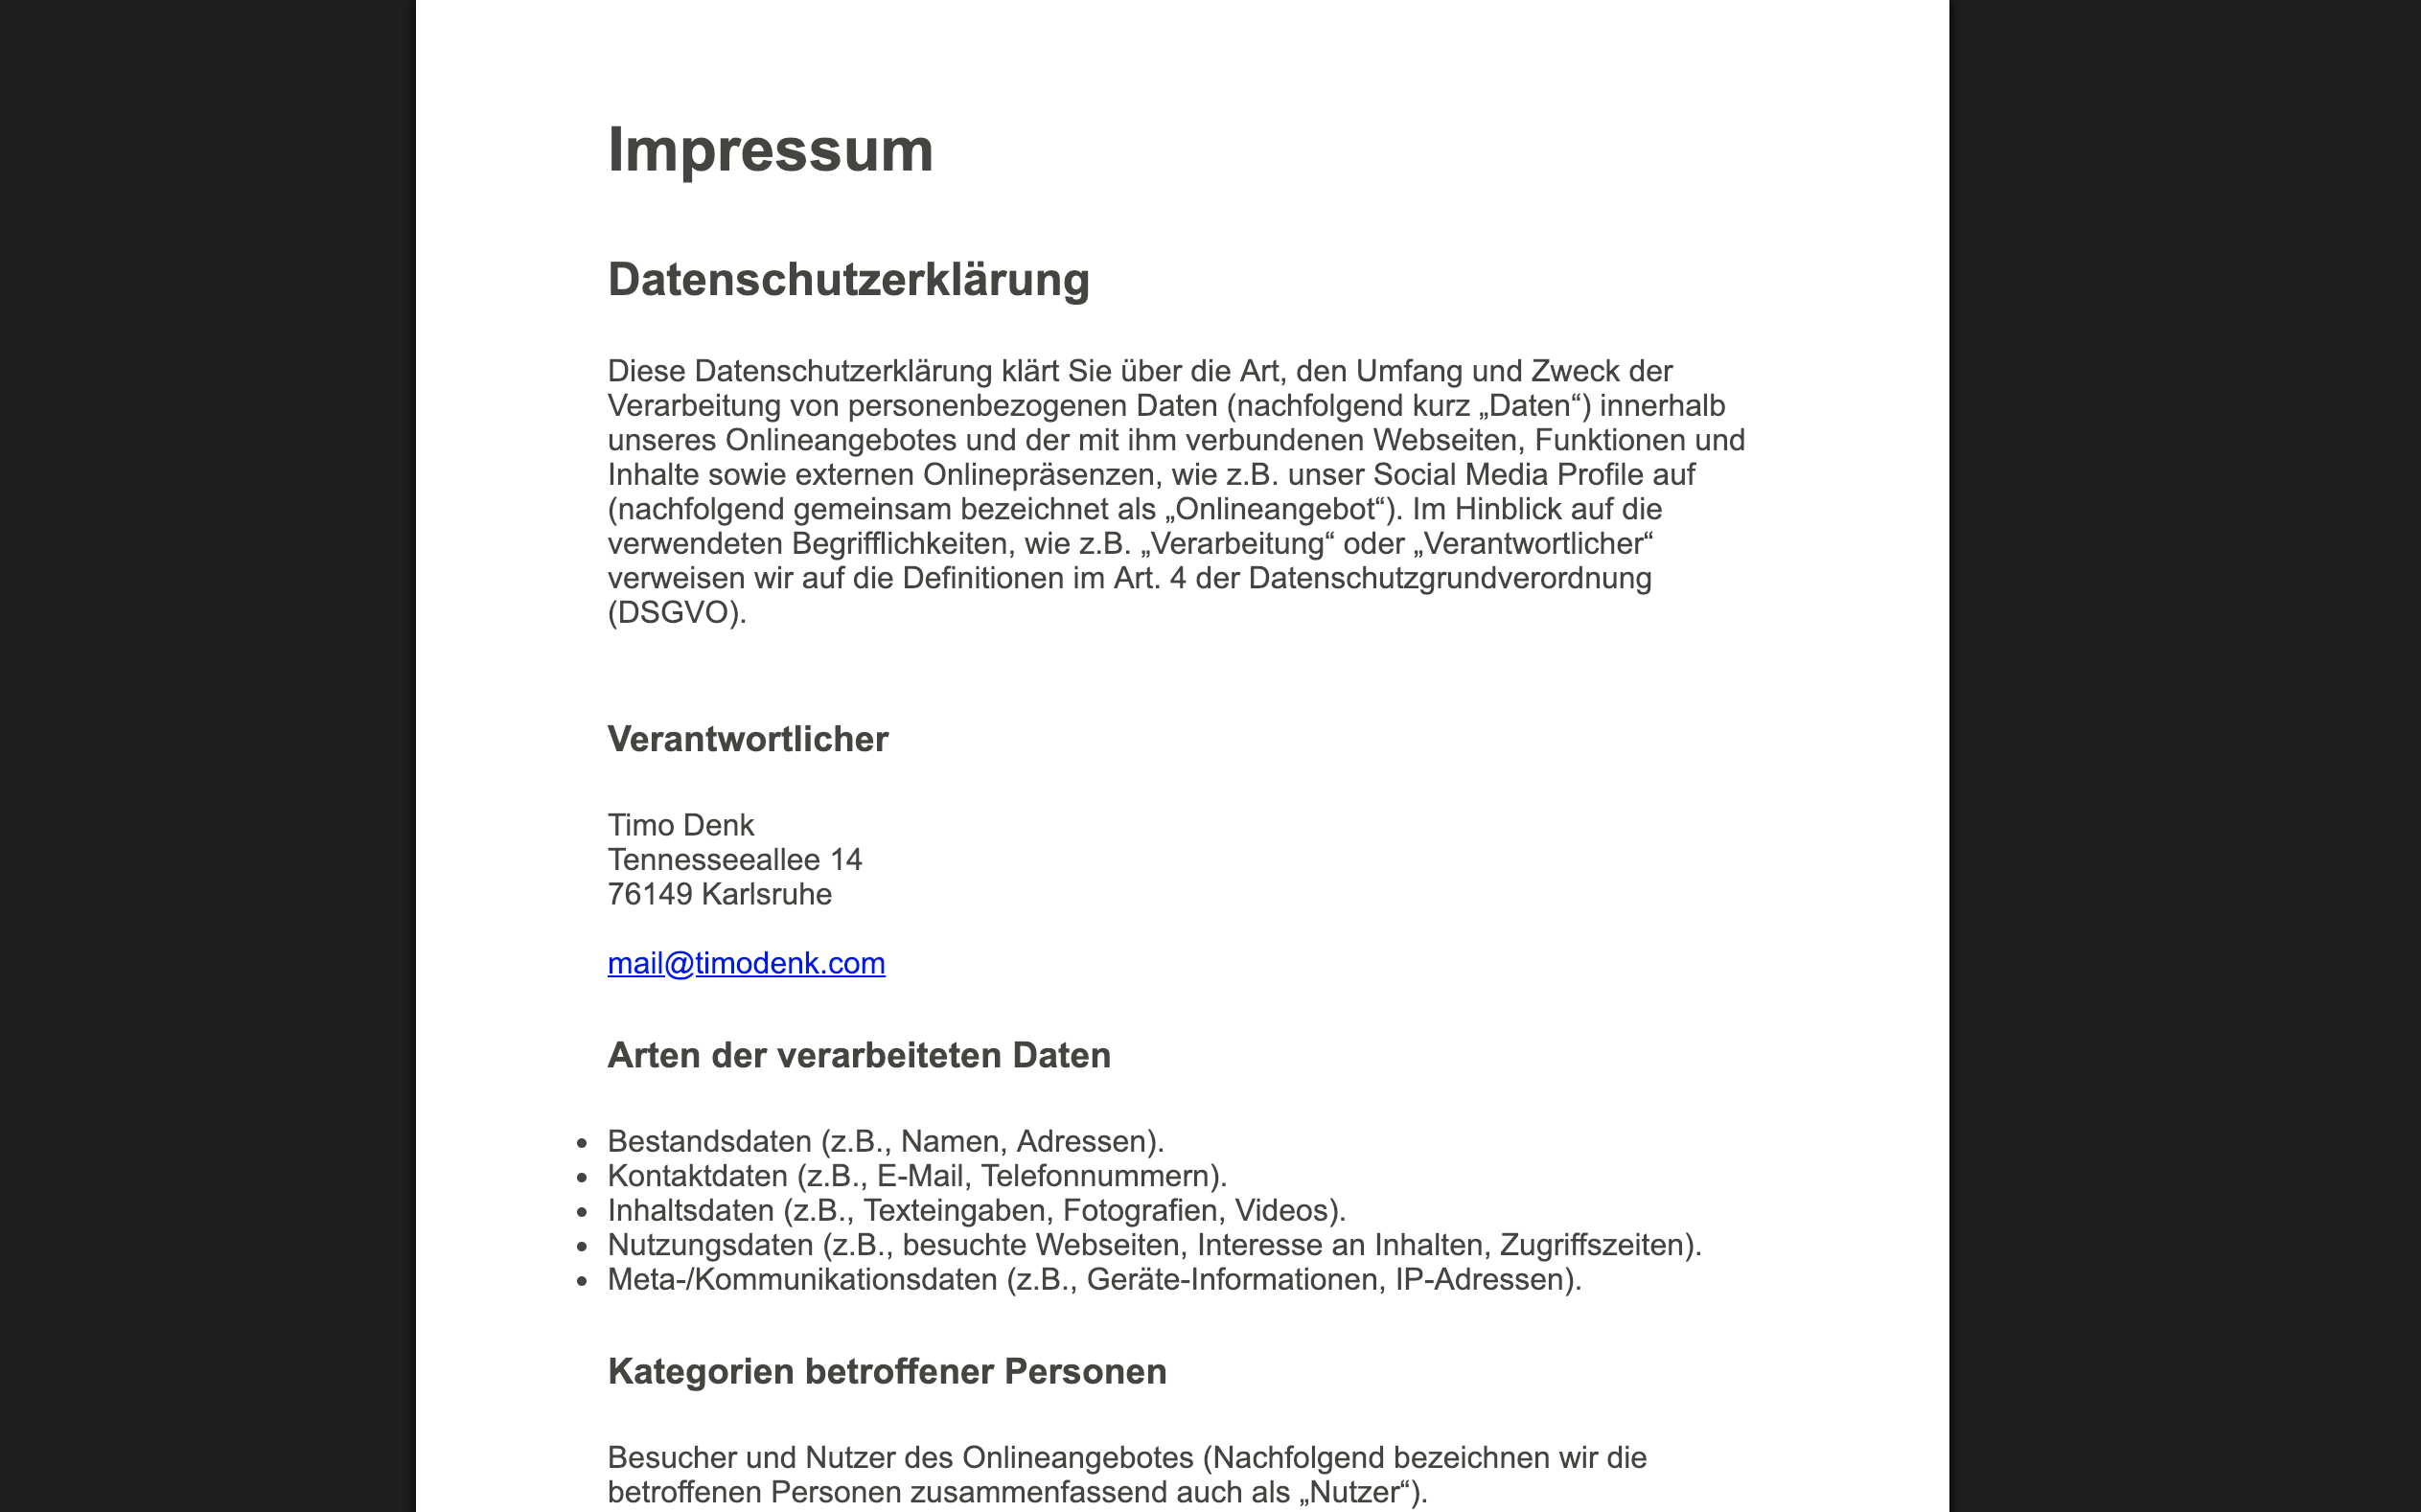
\includegraphics[width=.5\textwidth]{resources/imprint_timodenk}
\nodepart{three} 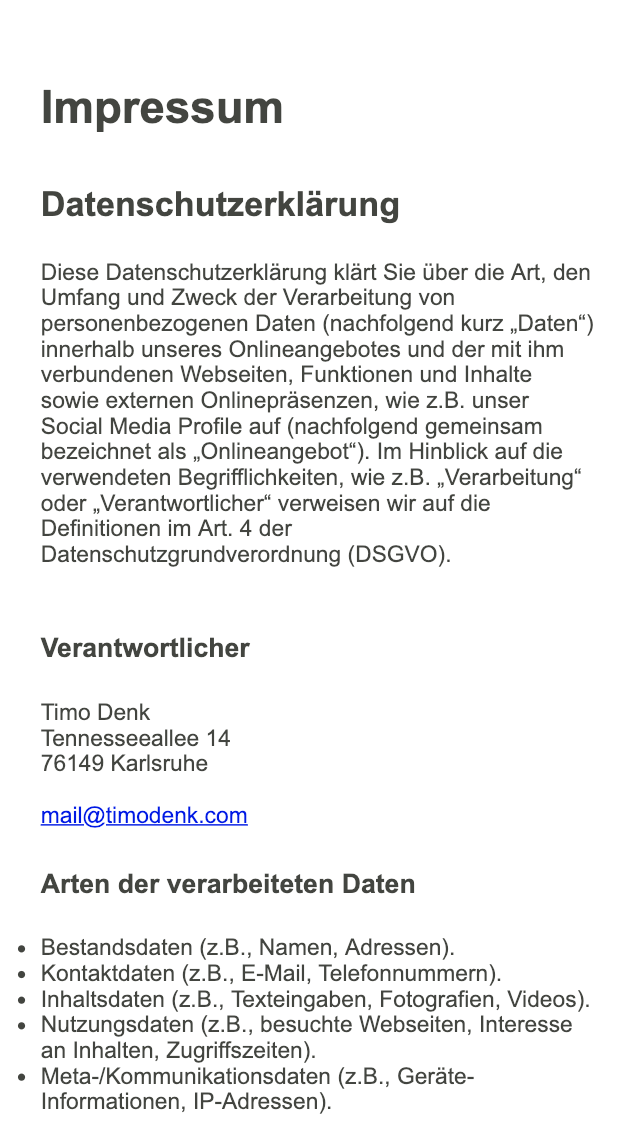
\includegraphics[width=.25\textwidth]{resources/imprint_timodenk_mobile}
\nodepart{four} Imprint - www.timodenk.com
\nodepart{five} 304 ms
\nodepart{six} 52 kb
};

\node (timodenkToImprint) at (0.5,6) {timodenk.com/imprint};
\node (timodenkToSites) at (9.5,6) {sites.timodenk.com};
\node (SitesToTimodenk) at (5.5,0.25) {timodenk.com};
\draw[-latex] (timodenk.one east) to [bend left=30] (sites.one north);
\draw[-latex] (sites.six west) to [bend left=30] (timodenk.six south);
\draw[-latex] (timodenk.one west) to [bend right=30](imprint.one north);
\end{tikzpicture}
}
\caption{Illustrates partial directed graph of domain \textit{timodenk.com} with three web pages, corresponding arrows and vertices}
\label{fig:PartialDirectedGraph_timodenk.com}
\end{figure}
